\documentclass[pdf]{beamer}
\usetheme{Berlin}
\usecolortheme{beaver}
%\mode<presentation>{}
\usepackage{amsmath}
\usepackage{tikz}
\usepackage{float}
\usepackage{pgfplots}
\usepackage{algorithm}
\usepackage{algorithmic}
\usepackage{bm}
\usepackage{cancel}
\usepackage{pgfplots}
%\usepackage{url}
%\usepackage[obeyspaces]{url}
\usepackage{hyperref}
\usepackage{subcaption}
\usetikzlibrary{shapes,snakes, patterns}

%% preamble
\title{Use of the 2D Navier-Stokes Equations to Explore Aerodynamic Properties of Trains}
\subtitle{ME EN 6720 Semester Projects}
\author{Christopher E. Mertin}
\date{April 29, 2016}
\begin{document}

%% title frame
\begin{frame}
\titlepage
\end{frame}
%% normal frame
\section{Background}

\begin{frame}{Motivation}
\begin{itemize}
\item Want to determine the optimal design of trains to mitigate drag
\end{itemize}
\end{frame}

\begin{frame}{Incompressible Flow Equations}
\begin{align}
u\frac{\partial u}{\partial x} + v\frac{\partial u}{\partial y} + \frac{1}{\rho}\frac{\partial P}{\partial x} &= \nu\nabla^{2}u\\
u\frac{\partial u}{\partial x} + v\frac{\partial u}{\partial y} + \frac{1}{\rho}\frac{\partial P}{\partial y} &= \nu\nabla^{2}v
\intertext{with the continuity equation being}
\frac{\partial u}{\partial x} + \frac{\partial v}{\partial y} &= 0
\end{align}
\end{frame}



\begin{frame}{Algorithm}
\begin{algorithm}[H]
\centering
\caption{Solving for the Primitive Variables}
\begin{algorithmic}
\WHILE{$\left|\left| P^{(n+1)} - P^{(n)}\right|\right|_{2} > tolerance$}
\STATE{Impose Boundary Conditions}
\STATE{$\vec{u}^{(t)} = \vec{u}^{(n)} + \Delta t \left(-\vec{A}^{(n)} + \vec{D}^{(n)}\right)$}
\STATE{$\nabla^{2}P^{(n+1)} = \frac{1}{\Delta t}\vec{\nabla}\cdot \vec{u}^{(t)}$}
\STATE{$\vec{u}^{(n+1)} = \vec{u}^{(t)} - \Delta t \nabla P^{(n+1)}$}
\STATE{$t = t + \Delta t$}
\ENDWHILE
\end{algorithmic}
\label{alg:navier_stokes}
\end{algorithm}
\end{frame}

\section{Boundary Conditions}
\begin{frame}{Boundary Conditions (Domain)}
\begin{figure}[H]
\centering
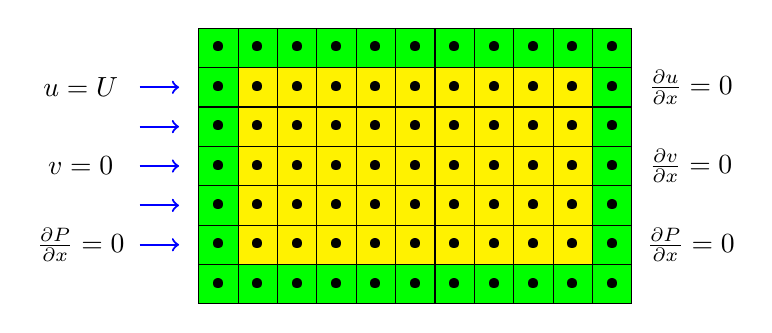
\begin{tikzpicture}[scale=0.5]
\draw[fill=green] (0,0) rectangle (11,7);
\draw[fill=yellow] (1,1) rectangle (10,6);
\draw (0,0) grid (11, 7);
\foreach \y in {0.5,...,6.5}
   \foreach \x in {0.5,...,10.5}
       \node at (\x,\y) {\textbullet};
\node at (12.5,5.5) {$\frac{\partial u}{\partial x} = 0$};
\node at (12.5,3.5) {$\frac{\partial v}{\partial x} = 0$};
\node at (12.5,1.5) {$\frac{\partial P}{\partial x} = 0$};
\node at (-3,5.5) {$u = U$};
\node at (-3,3.5) {$v = 0$};
\node at (-3,1.5) {$\frac{\partial P}{\partial x} = 0$};
\foreach \y in {1.5,...,5.5}
     \draw[blue,->,thick] (-1.5,\y) -- (-0.5,\y);
\end{tikzpicture}
\caption{Grid used in the computation. Green nodes denote the ``ghost nodes,'' while the yellow nodes cover the normal domain.}
\label{fig:grid}
\end{figure}
\end{frame}

\begin{frame}{Boundary Conditions (Train)}
We also needed to impose boundary conditions on the train to satisfy the {\em no-slip condition}. The no-slip condition requires that viscous fluids will have no velocity relative to a solid boundary. Therefore, to impose these conditions, we set both $u$ and $v$ to be $0$ on the interior of the train cars, and the following on their boundaries:
\begin{itemize}
\item Left and Right Faces: $\frac{\partial u}{\partial x} = 0$ and $v = 0$
\item Top and Bottom Faces: $\frac{\partial v}{\partial y} = 0$ and $u = 0$
\end{itemize}
\end{frame}

\begin{frame}{Grid Type}
The obvious choice of a grid is a collocated grid which stores $\{ P, u, v\}$ at each point in the grid. However, this causes problems with pressure--velocity coupling and the occurrence of oscillations in the pressure. Instead, the use of the staggered grid was chosen to overcome these irregularities. A diagram for a single node of this staggered grid can be seen in Figure~\ref{fig:stagg_1}.
\vspace{-1em}
\begin{figure}[H]
\centering
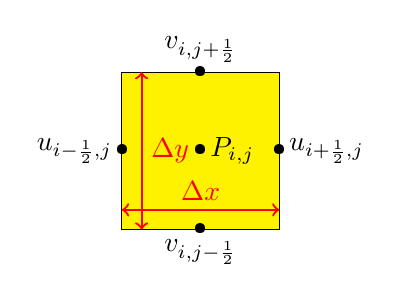
\begin{tikzpicture}[scale=0.5]
\draw [fill=yellow] (0, 0) rectangle (4,4);
\node at (0,2) {\textbullet};
\node at (2,2) {\textbullet};
\node at (4,2) {\textbullet};
\node at (2,0) {\textbullet};
\node at (2,4) {\textbullet};
\node [right] at (4,2) {$u_{i+\frac{1}{2},j}$};
\node [left] at (0,2) {$u_{i-\frac{1}{2},j}$};
\node [below] at (2,0) {$v_{i,j-\frac{1}{2}}$};
\node [above] at (2,4) {$v_{i,j+\frac{1}{2}}$};
\node [right] at (2,2) {$P_{i,j}$};
\node [right, red] at (0.5,2) {$\Delta y$};
\node [above, red] at (2,0.5) {$\Delta x$};
\draw [thick, red, <->] (0.5,0) -- (0.5,4);
\draw [thick, red, <->] (0, 0.5) -- (4, 0.5);
\end{tikzpicture}
\caption{Staggered Grid: Single Cell}
\label{fig:stagg_1}
\end{figure}
\end{frame}

\section{Verifying Simulations}

\begin{frame}{Verification of Simulation (cont.)}
\begin{figure}[h]
\centering
\includegraphics[width=.6\textwidth]{figs/pressure_single.pdf}
\caption{Typical plot for the pressure around a single block with $U=10$}
\end{figure}
\end{frame}

\begin{frame}{Verification of Simulation}
For simple problems, we can check to make sure that the code performs correctly. In doing so, we can derive an analytical solution for a simplified problem and test it for this case. We can do so using the {\em Reynold's Transport Theorem}  which is stated as

\begin{align}
\frac{\text{d}B}{\text{d}t} &= \frac{\partial}{\partial t}\int_{C_{v}}\rho b \text{d}V + \int_{C_{s}}\rho b \vec{u}\cdot \text{d}\vec{s}
\intertext{where $B$ is any property of the local system. For the pressure, this equation turns into}
\frac{\text{d}P}{\text{d}t} = \sum \vec{F} &= \cancel{\frac{\partial}{\partial t}\int_{C_{v}}\rho \vec{u} \text{d}V} + \int_{C_{s}}\rho \vec{u}\left( \vec{u}\cdot \text{d}\vec{A}\right)\label{eq:full_p}
\end{align}
\end{frame}

\begin{frame}{Verification of Simulation (cont.)}
\begin{align}
\intertext{with the first term going to zero due to conservation of flux. The forces that the train car are going to experience are the pressure $(F_{p})$ and the drag force $(F_{d})$. $F_{p}$ is defined as}
F_{p} &= -\int p \text{d}\vec{A}\label{eq:F_p}\\
F_{L} &= \oint p \cdot \hat{n}\ \text{d}A\label{eq:F_l}
\end{align}
\end{frame}

\begin{frame}{Verification of Simulation (cont.)}
\begin{align}
\intertext{where we can rearrange Equation~(\ref{eq:full_p}) to solve for $F_{d}$, giving}
F_{d} &= \int p\ \text{d}\vec{A} - \oint p \cdot \hat{n}\ \text{d}A + \int_{C_{s}}\rho \vec{u}\left( \vec{u}\cdot \text{d}\vec{A}\right)\label{eq:drag}
\end{align}
\pause
\begin{align}
\intertext{Exact:}
F_{d} &= \frac{1}{2}\rho u^{2} C_{D} A\label{eq:fd}
\end{align}
\end{frame}



\begin{frame}{Verification of Simulation (cont.)}
\begin{figure}[h]
\centering
\includegraphics[width=.6\textwidth]{figs/vorticity_single.pdf}
\caption{Typical plot of vorticity and streamfunction around a single block with $U=10$}
\end{figure}
\end{frame}

\begin{frame}{Verification of Simulation (cont.)}
\begin{figure}[h]
\centering
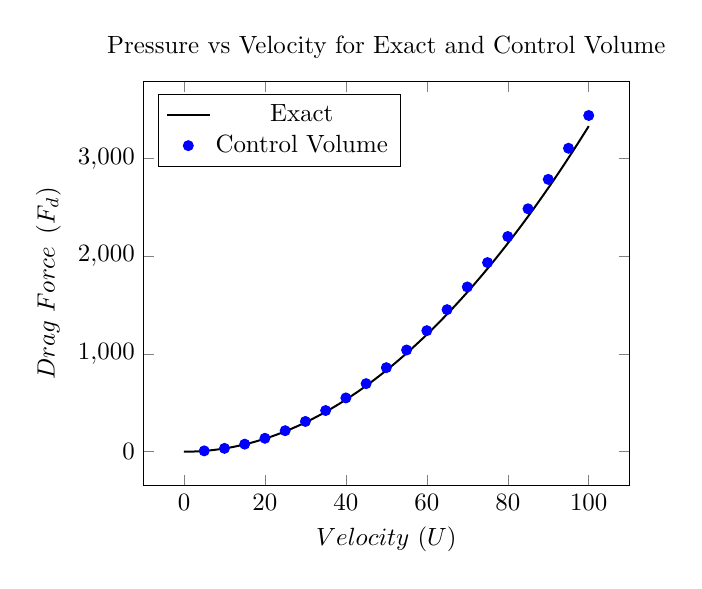
\begin{tikzpicture}[scale = 0.9]
\begin{axis}[xlabel={$Velocity\ (U)$}, ylabel={$Drag\ Force\ \left(F_{d}\right)$}, legend pos=north west, title={Pressure vs Velocity for Exact and Control Volume}]
\addplot[thick, color=black] coordinates{(0,0.000)(1,0.333)(2,1.333)(3,3.000)(4,5.333)(5,8.333)(6,12.000)(7,16.333)(8,21.333)(9,27.000)(10,33.333)(11,40.333)(12,48.000)(13,56.333)(14,65.333)(15,75.000)(16,85.333)(17,96.333)(18,108.000)(19,120.333)(20,133.333)(21,147.000)(22,161.333)(23,176.333)(24,192.000)(25,208.333)(26,225.333)(27,243.000)(28,261.333)(29,280.333)(30,300.000)(31,320.333)(32,341.333)(33,363.000)(34,385.333)(35,408.333)(36,432.000)(37,456.333)(38,481.333)(39,506.999)(40,533.333)(41,560.333)(42,587.999)(43,616.333)(44,645.333)(45,674.999)(46,705.333)(47,736.333)(48,767.999)(49,800.333)(50,833.333)(51,866.999)(52,901.332)(53,936.332)(54,971.999)(55,1008.332)(56,1045.332)(57,1082.999)(58,1121.332)(59,1160.332)(60,1199.999)(61,1240.332)(62,1281.332)(63,1322.999)(64,1365.332)(65,1408.332)(66,1451.999)(67,1496.332)(68,1541.332)(69,1586.998)(70,1633.332)(71,1680.332)(72,1727.998)(73,1776.332)(74,1825.332)(75,1874.998)(76,1925.331)(77,1976.331)(78,2027.998)(79,2080.331)(80,2133.331)(81,2186.998)(82,2241.331)(83,2296.331)(84,2351.998)(85,2408.331)(86,2465.331)(87,2522.997)(88,2581.331)(89,2640.331)(90,2699.997)(91,2760.331)(92,2821.331)(93,2882.997)(94,2945.330)(95,3008.330)(96,3071.997)(97,3136.330)(98,3201.330)(99,3266.997)(100,3333.330)};
\addlegendentry{Exact}
\addplot[color=blue, mark=*, only marks] coordinates{(5,8.608)(10,34.429)(15,77.464)(20,137.714)(25,215.178)(30,309.856)(35,421.748)(40,550.854)(45,697.174)(50,860.709)(55,1041.457)(60,1239.420)(65,1454.597)(70,1686.988)(75,1936.594)(80,2203.413)(85,2487.447)(90,2788.695)(95,3107.157)(100,3442.833)};
\addlegendentry{Control Volume}
\end{axis}
\end{tikzpicture}
\caption{Plot of the Pressure vs the Velocity on a single block}
\label{fig:p_vs_v}
\end{figure}
\end{frame}

\begin{frame}{Verification of Simulation (cont.)}
\begin{figure}[h]
\centering
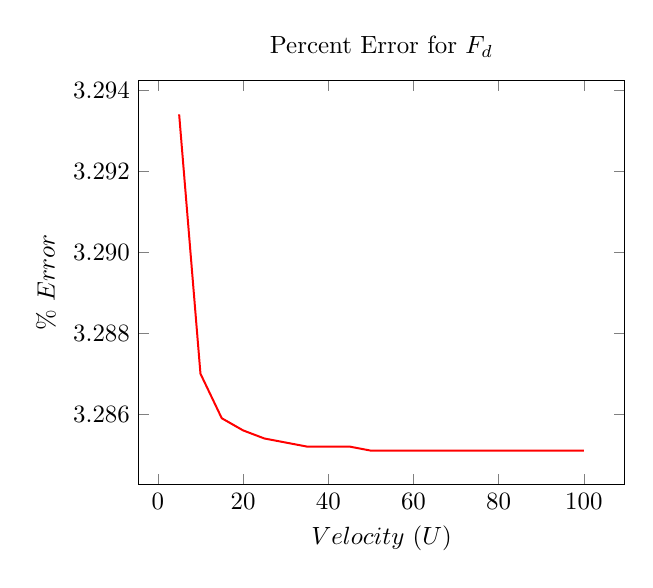
\begin{tikzpicture}[scale = 0.9]
\begin{axis}[xlabel={$Velocity\ (U)$}, ylabel={$\%\ Error$}, legend pos=north east, title={Percent Error for $F_{d}$}, y tick label style={/pgf/number format/.cd,fixed,fixed zerofill,precision=3,/tikz/.cd}]
\addplot[thick, color=red] coordinates{(5,3.2934)(10,3.2870)(15,3.2859)(20,3.2856)(25,3.2854)(30,3.2853)(35,3.2852)(40,3.2852)(45,3.2852)(50,3.2851)(55,3.2851)(60,3.2851)(65,3.2851)(70,3.2851)(75,3.2851)(80,3.2851)(85,3.2851)(90,3.2851)(95,3.2851)(100,3.2851)};
\end{axis}
\end{tikzpicture}
\caption{Plot of the Percent Error from the simulation}
\label{fig:p_error}
\end{figure}
\end{frame}

\section{Results}

\begin{frame}{Spacing Between Cars}
\begin{figure}[h]
\centering
\includegraphics[width=.6\textwidth]{figs/pressure_sep.pdf}
\caption{Pressure on the train for $U=10$ and $separation/width=11/15$}
\label{fig:p_sep}
\end{figure}
\end{frame}

\begin{frame}{Spacing Between Cars}
\begin{figure}[h]
\centering
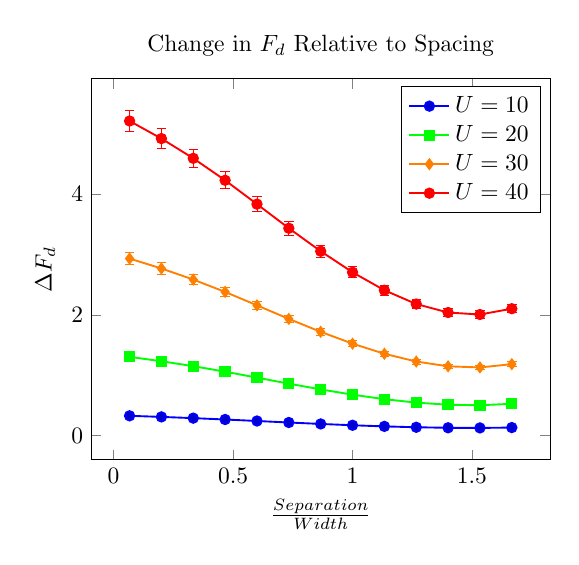
\begin{tikzpicture}[scale = 0.85]
\begin{axis}[xlabel={$\frac{Separation}{Width}$}, ylabel={$\Delta F_{d}$}, title = {Change in $F_{d}$ Relative to Spacing}]
\addplot+[thick, error bars/.cd, y dir=both, y explicit] coordinates{
(0.0667,0.3262) +- (0.0108,0.0108)
(0.2000,0.3081) +- (0.0102,0.0102)
(0.3333,0.2877) +- (0.0095,0.0095)
(0.4667,0.2650) +- (0.0087,0.0087)
(0.6000,0.2403) +- (0.0079,0.0079)
(0.7333,0.2153) +- (0.0071,0.0071)
(0.8667,0.1915) +- (0.0063,0.0063)
(1.0000,0.1696) +- (0.0056,0.0056)
(1.1333,0.1510) +- (0.0050,0.0050)
(1.2667,0.1366) +- (0.0045,0.0045)
(1.4000,0.1277) +- (0.0042,0.0042)
(1.5333,0.1255) +- (0.0041,0.0041)
(1.6667,0.1313) +- (0.0043,0.0043)
};
\addlegendentry{$U = 10$}
\addplot+[mark = square*, color = green, mark options=green, thick, error bars/.cd, y dir=both, y explicit] coordinates{
(0.0667,1.3030) +- (0.0430,0.0430)
(0.2000,1.2302) +- (0.0406,0.0406)
(0.3333,1.1485) +- (0.0379,0.0379)
(0.4667,1.0575) +- (0.0349,0.0349)
(0.6000,0.9587) +- (0.0316,0.0316)
(0.7333,0.8589) +- (0.0283,0.0283)
(0.8667,0.7637) +- (0.0252,0.0252)
(1.0000,0.6765) +- (0.0223,0.0223)
(1.1333,0.6020) +- (0.0199,0.0199)
(1.2667,0.5448) +- (0.0180,0.0180)
(1.4000,0.5095) +- (0.0168,0.0168)
(1.5333,0.5012) +- (0.0165,0.0165)
(1.6667,0.5252) +- (0.0173,0.0173)
};
\addlegendentry{$U = 20$}
\addplot+[mark=diamond*, color=orange, mark options=orange, thick, error bars/.cd, y dir=both, y explicit] coordinates{
(0.0667,2.9310) +- (0.0967,0.0967)
(0.2000,2.7670) +- (0.0913,0.0913)
(0.3333,2.5832) +- (0.0852,0.0852)
(0.4667,2.3785) +- (0.0785,0.0785)
(0.6000,2.1562) +- (0.0712,0.0712)
(0.7333,1.9317) +- (0.0637,0.0637)
(0.8667,1.7174) +- (0.0567,0.0567)
(1.0000,1.5214) +- (0.0502,0.0502)
(1.1333,1.3539) +- (0.0447,0.0447)
(1.2667,1.2252) +- (0.0404,0.0404)
(1.4000,1.1460) +- (0.0378,0.0378)
(1.5333,1.1276) +- (0.0372,0.0372)
(1.6667,1.1816) +- (0.0390,0.0390)
};
\addlegendentry{$U = 30$}
\addplot+[mark=*, color=red, mark options=red, thick, error bars/.cd, y dir=both, y explicit] coordinates{
(0.0667,5.2102) +- (0.1719,0.1719)
(0.2000,4.9187) +- (0.1623,0.1623)
(0.3333,4.5919) +- (0.1515,0.1515)
(0.4667,4.2279) +- (0.1395,0.1395)
(0.6000,3.8328) +- (0.1265,0.1265)
(0.7333,3.4337) +- (0.1133,0.1133)
(0.8667,3.0527) +- (0.1007,0.1007)
(1.0000,2.7042) +- (0.0892,0.0892)
(1.1333,2.4065) +- (0.0794,0.0794)
(1.2667,2.1778) +- (0.0719,0.0719)
(1.4000,2.0372) +- (0.0672,0.0672)
(1.5333,2.0044) +- (0.0661,0.0661)
(1.6667,2.1005) +- (0.0693,0.0693)
};
\addlegendentry{$U = 40$}
\end{axis}
\end{tikzpicture}
\caption{Plot of $F_{d}$ experienced by the second train car subtracted from $F_{d}$ on a single block}
\label{fig:fd_sub}
\end{figure}
\end{frame}

\begin{frame}{Spacing Between Cars}
\begin{figure}[h]
\centering
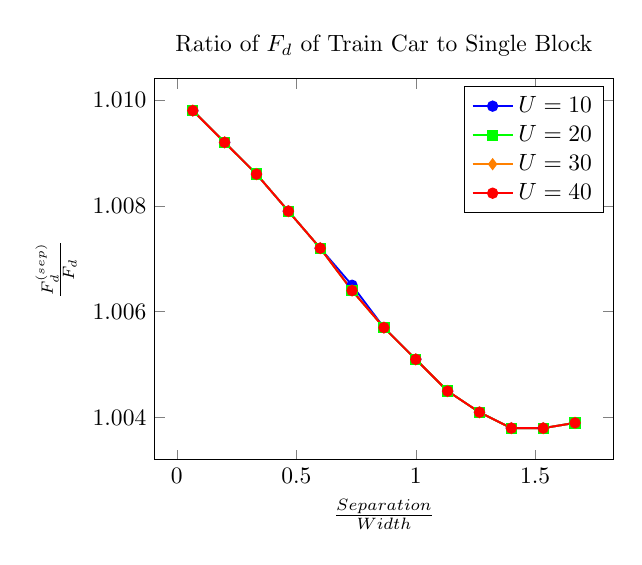
\begin{tikzpicture}[scale = 0.85]
\begin{axis}[xlabel={$\frac{Separation}{Width}$}, ylabel={$\frac{F_{d}^{(sep)}}{F_{d}}$}, title={Ratio of $F_{d}$ of Train Car to Single Block}, y tick label style={/pgf/number format/.cd,fixed,fixed zerofill,precision=3,/tikz/.cd}]
\addplot[mark=*, thick, color=blue] coordinates{
(0.0667,1.0098)
(0.2000,1.0092)
(0.3333,1.0086)
(0.4667,1.0079)
(0.6000,1.0072)
(0.7333,1.0065)
(0.8667,1.0057)
(1.0000,1.0051)
(1.1333,1.0045)
(1.2667,1.0041)
(1.4000,1.0038)
(1.5333,1.0038)
(1.6667,1.0039)
};
\addlegendentry{$U = 10$}
\addplot[mark=square*, thick, color=green] coordinates{
(0.0667,1.0098)
(0.2000,1.0092)
(0.3333,1.0086)
(0.4667,1.0079)
(0.6000,1.0072)
(0.7333,1.0064)
(0.8667,1.0057)
(1.0000,1.0051)
(1.1333,1.0045)
(1.2667,1.0041)
(1.4000,1.0038)
(1.5333,1.0038)
(1.6667,1.0039)
};
\addlegendentry{$U = 20$}
\addplot[mark=diamond*, thick, color=orange] coordinates{
(0.0667,1.0098)
(0.2000,1.0092)
(0.3333,1.0086)
(0.4667,1.0079)
(0.6000,1.0072)
(0.7333,1.0064)
(0.8667,1.0057)
(1.0000,1.0051)
(1.1333,1.0045)
(1.2667,1.0041)
(1.4000,1.0038)
(1.5333,1.0038)
(1.6667,1.0039)
};
\addlegendentry{$U = 30$}
\addplot[mark=otimes*, thick, color=red] coordinates{
(0.0667,1.0098)
(0.2000,1.0092)
(0.3333,1.0086)
(0.4667,1.0079)
(0.6000,1.0072)
(0.7333,1.0064)
(0.8667,1.0057)
(1.0000,1.0051)
(1.1333,1.0045)
(1.2667,1.0041)
(1.4000,1.0038)
(1.5333,1.0038)
(1.6667,1.0039)
};
\addlegendentry{$U = 40$}
\end{axis}
\end{tikzpicture}
\caption{Ratio between $F_{d}$ on the second train car to that of $F_{d}$ experienced on a single block}
\label{fig:fd_ratio}
\end{figure}
\end{frame}

\begin{frame}{Ground Clearance}
\begin{figure}[h]
\centering
\includegraphics[width=.6\textwidth]{figs/pressure_clearance.pdf}
\caption{Pressure on train for $U=10$ and $clearance/width = 1/3$}
\label{fig:clearance}
\end{figure}
\end{frame}

\begin{frame}{Ground Clearance}
\begin{figure}[h]
\centering
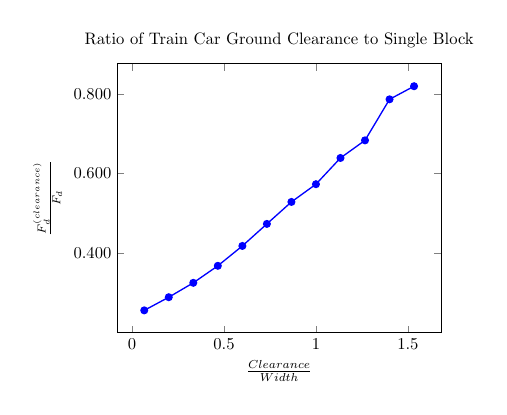
\begin{tikzpicture}[scale=.6]
\begin{axis}[xlabel={$\frac{Clearance}{Width}$}, ylabel={$\frac{F_{d}^{(clearance)}}{F_{d}}$}, title={Ratio of Train Car Ground Clearance to Single Block}, y tick label style={/pgf/number format/.cd,fixed,fixed zerofill,precision=3,/tikz/.cd}]
\addplot[mark=*, thick, color=blue] coordinates{
(0.0667,0.2568)
(0.2000,0.2898)
(0.3333,0.3259)
(0.4667,0.3686)
(0.6000,0.4184)
(0.7333,0.4737)
(0.8667,0.5288)
(1.0000,0.5733)
(1.1333,0.6391)
(1.2667,0.6833)
(1.4000,0.7862)
(1.5333,0.8191)
};
%\addlegendentry{$U = 10$}
\end{axis}
\end{tikzpicture}
\caption{Ratio of $F_{d}$ experienced on the second train car to that of a single block with $separation/width = 11/15$}
\label{fig:fdclear_fd}
\end{figure}
\end{frame}

\section{Conclusion}
\begin{frame}{Conclusion}
\begin{itemize}
\item Ground clearance is dominant factor
\item Spacing between cars is essentially negligable
\pause
\item Optimal Train:
\begin{itemize}
\item Low Diameter Wheels
\item Close spacing since $F_{d}$ is negligable ($1\%$ increase)
\item Conserve materials
\end{itemize}
\end{itemize}
\end{frame}

\end{document}

